%%===========================================================%%
%%                                                                                                                      %%
%%                                                    BAD RUNS                                                 %%
%%                                                                                                                      %%
%%===========================================================%%


\chapter{Bad run list}\label{chap:badRunList}

Diffractive analyses~\cite{AnalysisNoteRafal,AnalysisNoteLukasz} were performed with the use of data from runs with completion status ``Successful'' in the STAR run log~\cite{RunLog}. During analysis of these runs no problems with the reconstructed data were found. The distributions of the TPC track-related quantities and performance of remaining subsystems used in analyses did not indicate issues preventing this data from inclusion to physics analyses.

On top of above we omitted from analyses data taken with Roman Pot detectors far from their nominal positions. By the nominal position we understand the vertical distance between the nominal beam trajectory and the closest edge of the Silicon Strip Detector housed inside Roman Pot. This positions were first measured during dedicated survey~\cite{surveyNote} and later precisely calculated for all runs and for all detectors using elastic proton-proton scattering events~\cite{alignmentPresentation,alignmentDirectory}.%~\cite{alignmentPresentation, alignmentNote, alignmentDirectory}.

Below we show histogram (Fig.~\ref{fig:positionHistograms}) and graph (Fig.~\ref{fig:positionVsRunGraph}) of the beam-detector positions of all Roman Pots during runs with active RP triggers\footnote{Roman Pots were not moved during the run. They were only moved between the runs.}. Based on these plots we set the limit of the nominal position of the detector with respect to the beam to $y_{\text{thr}} =$~34~mm. If any of 8 detectors was further from the beam than the threshold ($|y|>y_{\text{thr}}$) the run run was omitted from analysis. The benefit of that selection was reduction of the systematic effects related to low/asymmetric acceptance of detectors when they are at far/significantly differing distances from the nominal beam trajectory.

In the Fig.~\ref{fig:rpPosition} one can notice that there were a few runs (16106026-16106033, fill 18915) with the closer-than-nominal distance of detectors to the beamline. These runs correspond to a period when an enhanced sample of RP\_ET triggers was collected, dedicated for a study of elastic proton-proton scattering. There is no significant difference in beam conditions that these data were taken with. The main characteristics is that there were multiple vernier scans conducted during the RHIC fill for better precision in luminosity determination. Although detector position differs from the nominal for these few runs, the active area of Roman Pots still covered the fiducial area defined for a physics measurement. We therefore preserve these runs for all analyses. 

%--------------------------
\begin{figure}[hb]
\centering
\parbox{0.4\textwidth}{
  \centering
  \begin{subfigure}[b]{\linewidth}{
                \subcaptionbox{\label{fig:positionHistograms}}{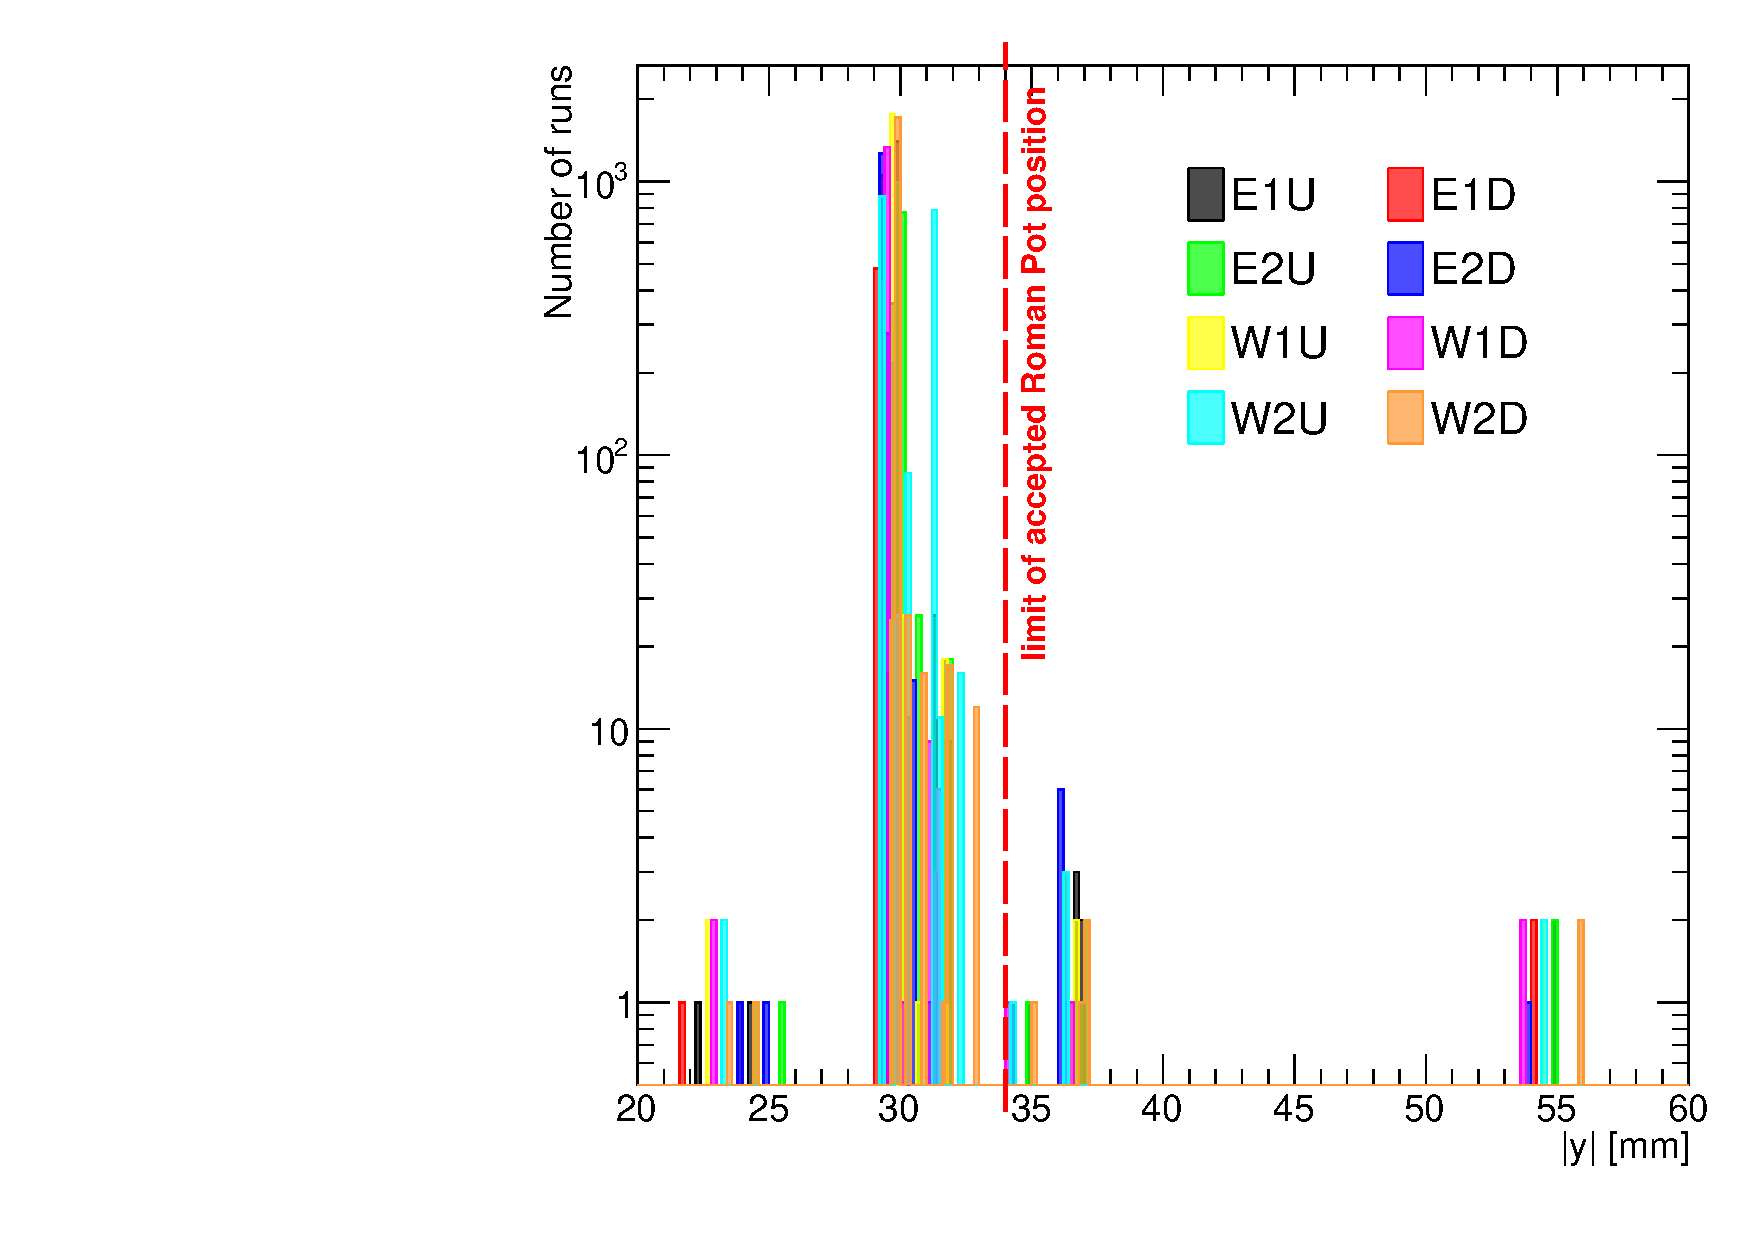
\includegraphics[width=\linewidth]{graphics/badRuns/positionHistograms.pdf}}}
  \end{subfigure}
}
\quad
\parbox{0.545\textwidth}{
  \centering
  \begin{subfigure}[b]{\linewidth}{
                \subcaptionbox{\label{fig:positionVsRunGraph}}{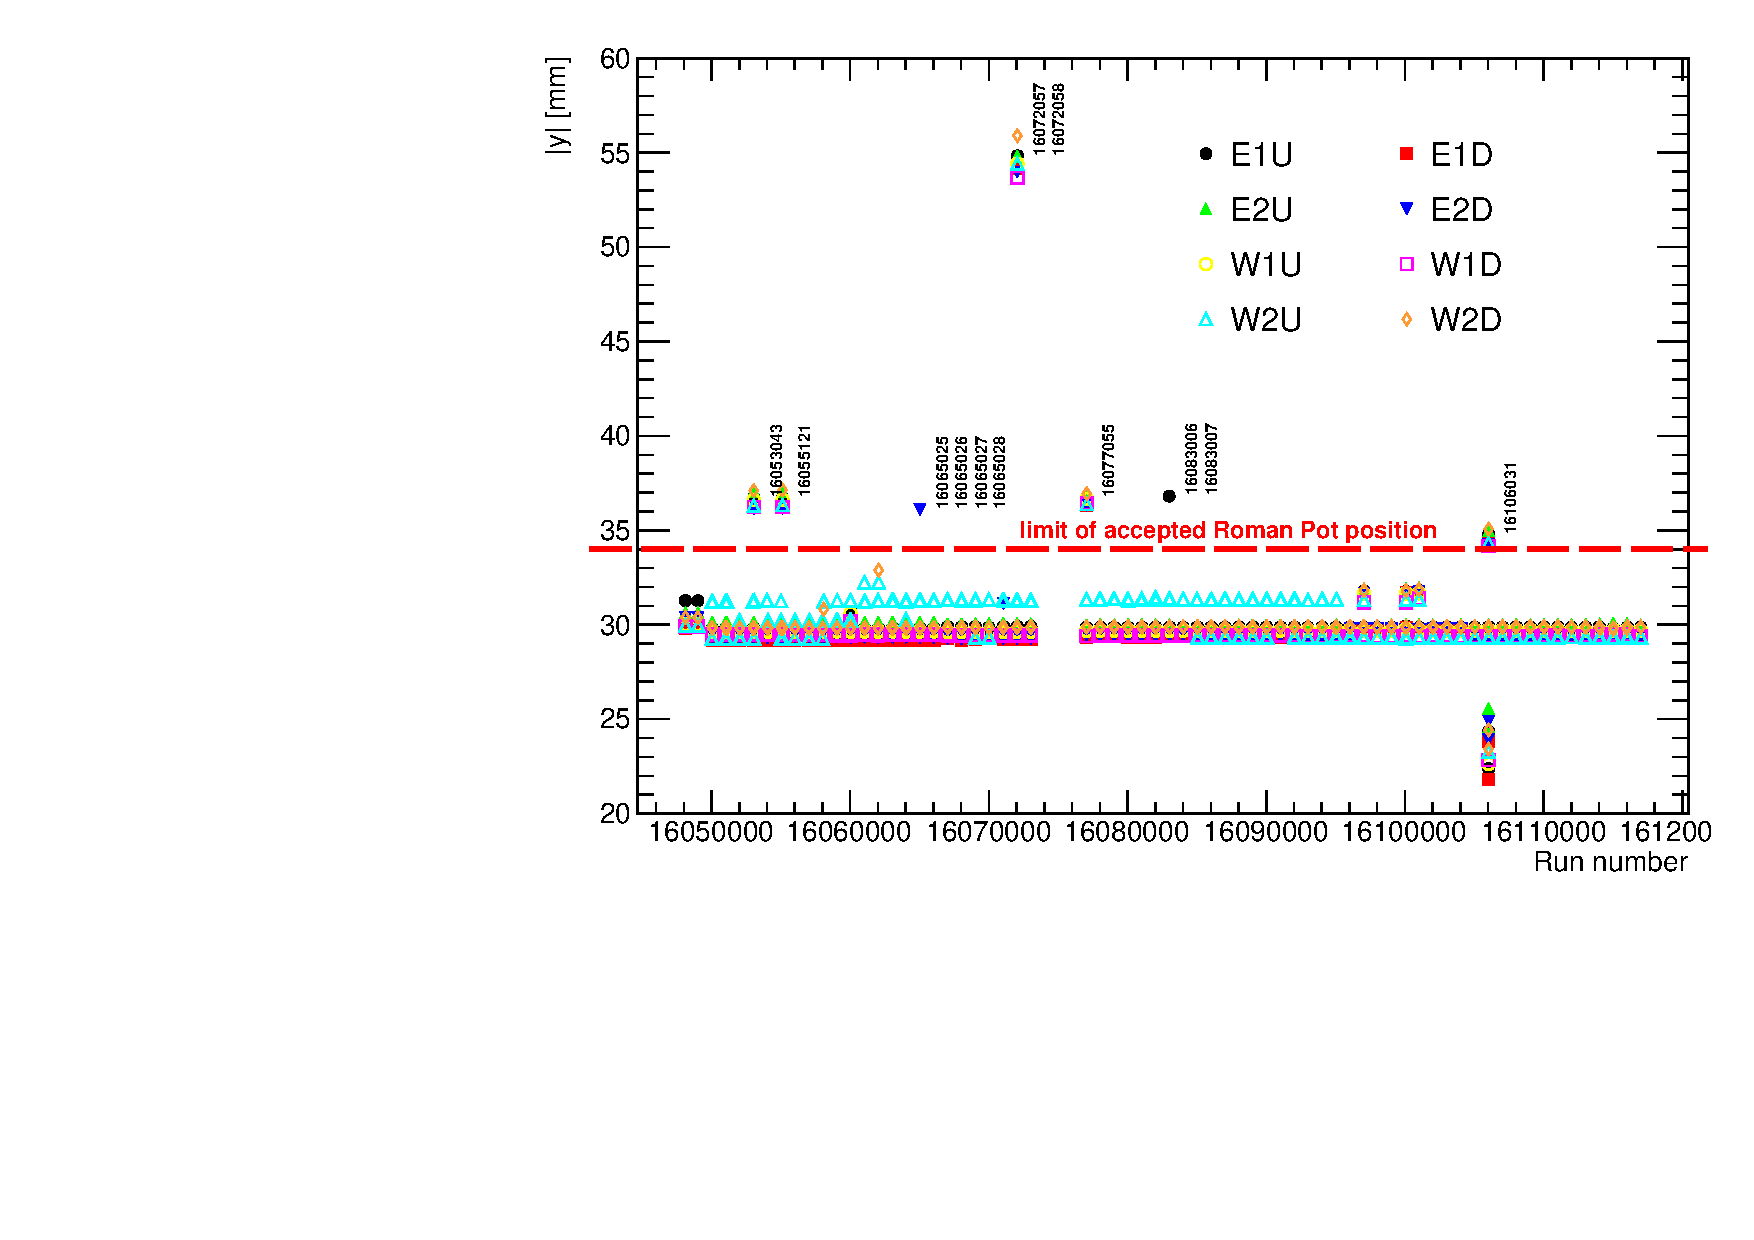
\includegraphics[width=\linewidth]{graphics/badRuns/positionVsRunGraph.pdf}}}
  \end{subfigure}
}%
\caption[Beam-detector distance of the Roman Pots in run 15.]{Histogram of beam-detector distance $|y|$ (\ref{fig:positionHistograms}) and graph showing run-dependence of $|y|$ (\ref{fig:positionVsRunGraph}) for all Roman Pots.}\label{fig:rpPosition}
\end{figure}
%---------------------------

A summary list of runs in which detector positions did not fulfill beam-detector distance limits are listed below:%
%
\begin{center}
\begin{tabular}{llllll}
16053043 & 16055121 & 16065025 & 16065026 & 16065027 & 16065028\\
16072057 & 16072058 & 16077055 & 16083006 & 16083007 & 16106031\\
\end{tabular}
\end{center}%
%
Full list of runs with diffractive triggers (``RP\_xxxx'') and the list of runs for each trigger can be found at the web adress given in Ref.~\cite{onlineRpTriggersMonitoring}.